\section{Développement de l'application}

\indent L'application finale demandée reprend les éléments de configuration vus en section 2.
Cette section comporte un récapitulatif des éléments de l'application avec des portions de code montrant leur utilisation.
Un exemple de résultats obtenus après lancement de l'application sont montrés.

\subsection{Cahier des charges}

\indent Il s'agit d'implanter une application simple permettant de mesurer le temps de réaction d'une personne (Utilisateur) et mettant en œuvre différentes entrées/sorties disponibles sur la carte SAMD21 en utilisant SW0 et LED0 et sur la carte OLED1 (extension de la carte SAMD21) en utilisant BP1, BP2, BP3, LED1, LED2, LED3 et l'écran OLED.
La structure fonctionnelle de l'application à développer peut être présentée dans un premier temps (légèrement modifiée par la suite) par la figure suivante :

\begin{figure}[h]
    \centering
    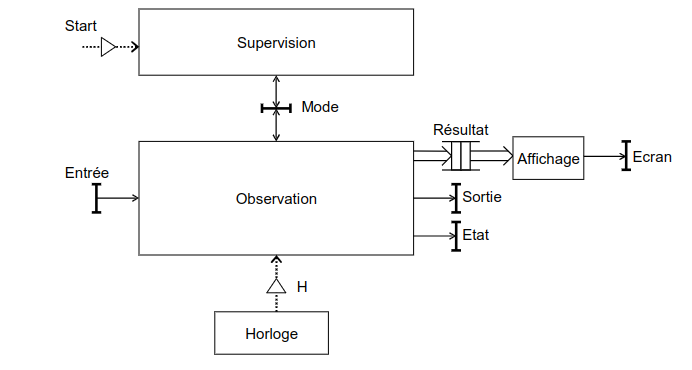
\includegraphics[width=0.7\linewidth]{struct_fonc.png}
    \caption{Structure fonctionnelle initiale de l'application à développer}
    \label{fig:struct}
\end{figure}
 La mesure de vitesse de réaction est démarrée lors de l'apparition de l'événement Start.
Elle consiste alors à émettre un code aléatoire en allumant un ensemble de LED (variable Sortie matérialisée par LED1, LED2 et LED3) et à mesurer le temps nécessaire à l'utilisateur pour reproduire la combinaison sur des boutons poussoirs (variable Entrée, matérialisée par BP1, BP2 et BP3) en comptant le nombre d'événements H entre la production d'une valeur sur Sortie et la reproduction de cette valeur sur Entrée. 
Plusieurs mesures de vitesse de réaction peuvent être effectuées afin d'obtenir des valeurs minimale, moyenne et maximale.
Dans le programme, la constante \texttt{NbMesToDo} est fixée à 5 à titre d'exemple.
L'utilisateur verra sont temps de réaction mesuré 5 fois.
Lorsque toutes les mesures sont effectuées, des statistiques sont transmises à la fonction Affichage qui se charge de les afficher sur l'Ecran de la carte OLED1.
La précision de la mesure du temps de réaction doit être de 1 ms.
L'état de la fonction d'observation (Observe ou Non\_Observe) est en permanence affiché (variable Etat, matérialisée par LED0 de la carte SAMD21XPLAINEDPRO, la LED0 doit être allumée lorsque Etat a la valeur Observe).
Le comportement de la fonction Observation est défini par l'automate de la figure \ref{fig:automate}.


\subsection{Éléments de l'application}

L'application se base sur la structure fonctionnelle suivante :

\begin{figure}[h]
    \centering
    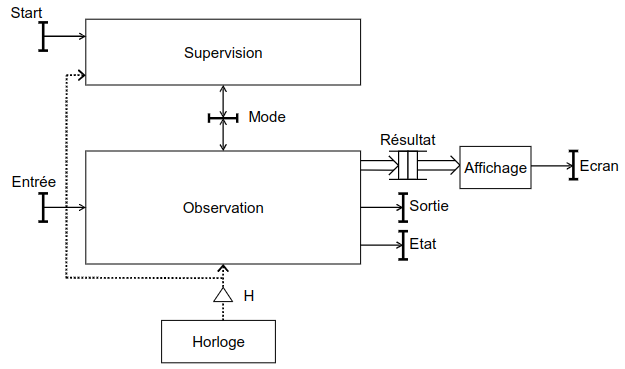
\includegraphics[width=0.7\linewidth]{struct_fonc_final.png}
    \caption{Structure fonctionnelle de l'application à développer}
    \label{fig:struct_final}
\end{figure}

Par rapport à la structure fonctionnelle présentée en figure \ref{fig:struct}, \textit{Start} n'est plus un évènement mais une variable partagée.
Cette solution est plus simple à implanter car elle ne nécessite pas la gestion des interruptions engendrée par l'attente d'un évènement en entrée du système.
De ce schéma, différentes informations peuvent être extraites.
Quatre tâches distinctes peuvent être imaginées pour cette application temps-réel: Horloge, Supervision, Observation et Affichage.
Deux sémaphores, matérialisées l'évènement H, sont nécessaires pour synchroniser les têches Supervision" et "Observation".
L'application contient une variable partagée \textit{Mode} et une file de message \textit{Résultats}.
Les différentes entrées/sorties présentées dans cette structure fonctionnelle correspondent à des éléments physiques présents sur la carte tels que des boutons poussoirs, des LEDs ou l'écran.

\subsection{Code de l'application}
L'application a été développée sur l'environnement Microchip Studio.
Cet environnement est adapté au développement d'une application temps-réel et nécessite deux machines : le post de développement et la cible embarquée.
Il est en effet équipé d'une chaîne de cross-compilation et peut programmer la cible via une liaison série.
Il est également équipé d'un outil de debug.
Dans le cadre du projet, la cible est une carte SAMD21XPLAINEDPRO et sa carte d'extension OLED1XPLAINEDPRO.
La cible recevra l'application tournant sur un exécutif temps-réel FreeRTOS.
Au long des séances de projet, l'exécutif temps-réel FreeRTOS a été configuré de sorte à pouvoir recevoir l'application.
Il est par exemple possible, après modification du fichier FreeRTOSConfig.h, de modifier l'horloge de référence du CPU reçue par FreeRTOS.
Dans le cadre du projet, l'horloge de référence a une fréquence de 8 MHz.
% De plus, il est possible de définir le nombre de Ticks d'horloge par seconde envoyé par FreeRTOS aux applications.
% Ici, l'OS envoie 1000 Ticks/secondes soit une fréquence de 1 kHz.
% La gestion des horloges au sein du système peut être résumée ainsi:

% \begin{figure}[h]
%     \centering
%     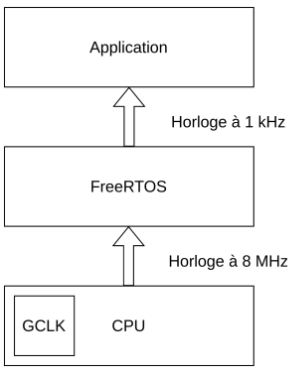
\includegraphics[width=0.7\linewidth]{horloges.png}
%     \caption{Configuration des horloges pour l'application}
%     \label{fig:clock}
% \end{figure}

Enfin, il est possible de modifier la taille de pile allouée à l'application.
Par défaut cette taille est de 60.
Progressivement, au fil des séances, des éléments sont ajoutés à l'application, notamment la gestion de l'écran OLED.
Une profondeur de pile de 60 n'est pas suffisante pour supporter la bibliothèque de l'écran, cette taille doit être réajustée.
Pour la suite du projet, la taille a été définie à 100.
Cette taille n'a pas été raffinée, mais en vue d'obtenir une application plus performante, la taille minimale nécessaire pourrait être trouvée.
L'application contient la définition des quatre tâches vues précédemment, des variables globales, des variables partagées, des sémaphores et de la file de message.
Les différents éléments sont créés et l'ordonnanceur est démarré dans la fonction \texttt{main()}.
Chaque tâche a une priorité qui lui est propre et un comportement précisé dans le corps du sujet.
Dans un premier temps, le comportement de chaque tâche est défini en accord avec la structure fonctionnelle (figure \ref{fig:struct_final}).

\subsubsection{Horloge}
La tâche Horloge est envoi deux sémaphores de synchronisation.
Un premier, nommé \texttt{H1}, est adressé à la tâche Observation et un second, \textit{H2}, à la tâche Supervision.
Au préalable, elle contient un appel à la procédure vTaskDelay qui correspond à une attente en Tick d'horloge.
Par défaut, ce nombre est défini à 1 et ne changera pas pour la suite du projet.

\subsubsection{Observation}
La tâche Observation est éveillé par le sémaphore \textit{H1} en provenance de la tâche Horloge.
Cette tâche implémente un automate bien défini dans le cahier de charge.
La figure \ref{fig:automate}, illustre le comportement spécifié.

\begin{figure}[h]
    \centering
    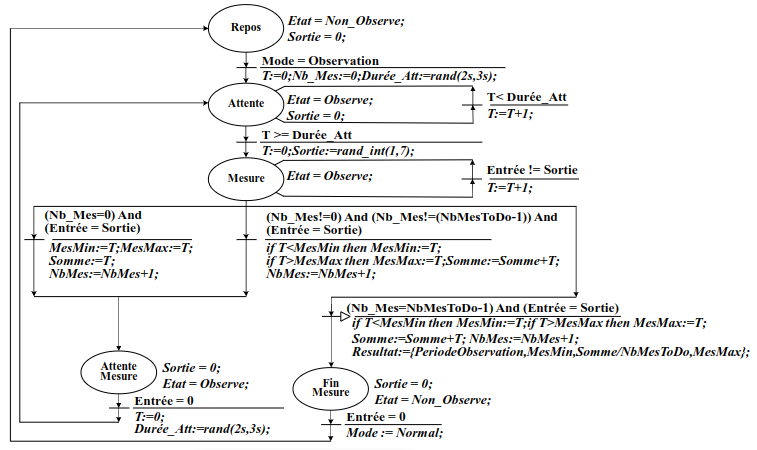
\includegraphics[width=0.9\linewidth]{automate_obs.png}
    \caption{Automate de la tâche Observation}
    \label{fig:automate}
\end{figure}

C'est la tâche Observation qui effectue les mesures du temps de réaction.
Pour démarrer une série de mesures, l'état de la variable partagée \textit{mode} est testé dans l'état initial de repos.
Lorsque \textit{mode} est égale à \texttt{Observation}, la série de mesures démarre.
À chaque mesure, les LED sont allumée selon une séquence aléatoire et le chronomètre est lancé.
Le temps tourne jusqu'à l'égalité avec les boutons.
La valeur temporelle mesurée est sauvegardé pour établir les statistiques.
Une nouvelle séquence commence si le nombre de mesures n'est pas atteint.
Lors de la dernière mesure, les performances de l'utilisateur sont envoyées à travers une file de message Résultats à la tâche Affichage.
Une structure de message est déclarée pour profiter de cette fonctionnalité disponible grâce à la file.
\begin{lstlisting}[style=CStyle]
typedef struct { /* Definition de la structure du message */
	uint16_t periodeObservation;
	uint16_t MesMin;
	uint16_t Moyenne;
	uint16_t MesMax;
} Resultat_t;
\end{lstlisting}
La tâche Affichage reçoit alors les données en un seul message.

\subsubsection{Supervision}
La tâche Supervision est, comme la tâche Observation, éveillé par un sémaphore en provenance de la tâche Horloge.
Cette tâche écrit sur la variable partagée \textit{mode} lorsque le bouton BP0 est appuyé, permettant de démarrer l'application.
L'algorithme en pseudo code issu du cahier des charges de la tâche observation est le suivant :
\begin{lstlisting}[frame=single, basicstyle = \ttfamily \footnotesize]
action Supervision() sur evenement H avec (Entree Var Start : (Appuye, Relache),
    Entree/Sortie Var Mode : (Normal, Observation)) ;
    Var StartPrec : (Appuye, Relache) ;
begin
    cycle H
    begin
        ReadState(Start); // lecture etat du BP Start
        if (StartPrec = Relache) & (Start=Appuyee & (Mode = Normal)) then
            Mode := Observation ;
            StartPrec := Start;
        end;
    end_cycle;
end_Supervision;
\end{lstlisting}
La condition au centre ce cette fonction permet démarrer une séquence de mesure en vaillant que la précédente soit bien achevée.


\subsubsection{Affichage}
La tâche Affichage est activée sur réception de la file de message Résultats en provenance de la tâche Observation.
Les résultats sont lus puis affichés sur l'écran.
La fonction \texttt{itoa} assure la conversion d'une valeur numérique en chaine de caractère.
Ensuite la bibliothèque de l'écran fournie une fonction prenant en entrée cette même chaine.
\begin{lstlisting}{style=CStyle}
    itoa(resultat.MesMin, str_val, 10);
	gfx_mono_draw_string(str_val, 75, 0, &sysfont);
\end{lstlisting}
Le texte en positionné aux coordonnées (75,0) soit centrée en haut.

Les quatre tâches doivent cohabiter sur le même système.
Il faut donc leur accorder une priorité.
Pour rappel, la politique d'ordonnancement de FreeRTOS est "préemptif à priorités fixes".
On applique la logique d'accorder la plus haute priorité aux tâches ayant l'activation les plus fréquentes.
Dans le cadre de l'application développé, les priorités de chaque tâche sont définies ainsi:
\begin{lstlisting}[style=CStyle]
    #define CLOCK_TASK_PRIORITY ( tskIDLE_PRIORITY +5 ) 
    #define OBSERVATION_TASK_PRIORITY ( tskIDLE_PRIORITY +2 )
    #define SUPERVISION_TASK_PRIORITY ( tskIDLE_PRIORITY +3 )
    #define AFFICHAGE_TASK_PRIORITY ( tskIDLE_PRIORITY +1 )
\end{lstlisting}
La tâche la plus prioritaire est logiquement l'horloge puisqu'elle envoie les sémaphores nécessaires à l'éveil des autres tâches.
La tâche Supervision est plus prioritaire que la tâche Observation puisqu'elle écrit sur la variable partagée \textit{mode} qui est lue dans la tâche Observation.
Enfin, la tâche Affichage est la moins prioritaire puisqu'elle reçoit une file de message de la tâche Observation.
C'est aussi cette dernière qui demande le plus de ressources de calcul.
Il est préférable que son exécution soit préemptée par les autres tâches.

\subsection{Résultat}

L'application peut être testée en programmant la carte.
L'utilisateur doit appuyer sur le bouton SW0 pour lancer une série de mesures du temps de réaction.
Dans le cadre des résultats montrés ci-dessous, cinq mesures successives sont effectuées avant l'affichage des résultats sur l'écran.
Les figures suivantes montrent l'affichage de l'écran au lancement de l'application (figure \ref{fig:start_app}) et à la fin d'une série de mesures (figure \ref{fig:end_app}).
Les résultats montrés sont, dans l'ordre le temps de réaction minimal, le temps de réaction moyen, le temps de réaction maximal et la période d'observation entre deux appels de la tâche Observation.
L'unité de chacune de ces valeurs est le \textit{tick d'horloge}.
\begin{figure}[H]
    \centering
    \begin{subfigure}[b]{0.3\textwidth}
        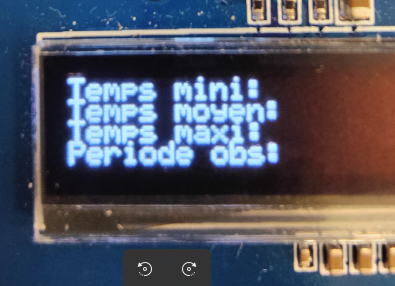
\includegraphics[width=\linewidth]{start_app.png}
        \caption{Affichage au lancement}
        \label{fig:start_app}
    \end{subfigure}
    \begin{subfigure}[b]{0.50\textwidth}
        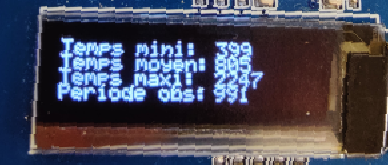
\includegraphics[width=\linewidth]{end_app.png}
        \caption{Affichage après mesures}
        \label{fig:end_app}
    \end{subfigure}
\end{figure}
Au lancement de l'application, l'écran affiche du texte en préparation de l'arrivée des résultats.
C'est lors de l'initialisation du matériel que cet affichage a lieu.
Après une série de mesures, la file de message contenant les résultats est envoyée de la tâche \textit{Observation} à la tâche \textit{Affichage}.
Cette file de message contient la variable \texttt{Résultat}, instance de la structure \texttt{Resultat\_t} contenant les différentes mesures.
Après réception de la file de message, la tâche \textit{Affichage} fait apparaître sur l'écran les résultats de la mesure.

Pour prouver le bon fonctionnement de l'application, une vidéo est proposée dans le même dossier que ce rapport.
Cette vidéo couvre le démarrage de l'application après un reset. 
Une série de mesures a lieu, menant à l'affichage des résultats.
Enfin, l'utilisateur relance une série de mesures après appui sur le bouton SW0.
Outre l'aspet fonctionnel de l'application, il est nécessaire de prouver son bon fonctionnement d'un point de vue temps-réel.
La mesure de la période d'obsevation permet de justifier que les tâches s'exécutent dans une fenêtre de temps qui respecte les contraintes temporelles.
La tâche "Observation" est réveillée par une sémaphore en provenance de la tâche "Clock".
Selon la configuration du projet, l'horloge définie par l'OS pour les applications est de 1 khHz.
La tâche "Clock" envoie un sémaphore d'éveil après une attente de 1 Tick d'horloge.
La tâche "Observation" devrait donc être réveillée environ tout les 1000 Ticks d'horloge.
Lors des tests effectués, c'est ce qui a pu être observé, avec une valeur de période d'observation toujours comprise entre 990 et 994.
Dans le cas des résultats présentés en figure \ref{fig:end_app}, la période d'observation est de 991 Ticks d'horloge.